%%%%%%%%%%%%%%%%%%%%%%%%%%%%%%%%%%%%%%%%%%%%%%%%%%%%%%%%%%%%%%%%%%%%%%%%%%%%%%%%
\documentclass[presentation]{beamer} %\mode<presentation>{\usetheme{sapere}}
\usepackage{talk-2025-telmed-nesy}

	
\title[NeSy AI for Chronic Disease]{
    % same title of the presented paper
    Neuro-symbolic AI for Supporting
    \\
    Chronic Disease Diagnosis and Monitoring
}
\subtitle{}
\author[MCKSM]{
	Matteo Magnini$^{*}$
	\and 
	Giovanni Ciatto$^{*}$
	\and
	Ahmet Emre Kuru$^{\dagger}$
	\\
	Christel Sirocchi$^{\ddagger}$
    \and
    \emph{Sara Montagna}$^{\ddagger}$
}
%
\institute[UniBo, Uni*]{
    $^{*}$\textsc{Alma Mater Studiorum} -- University of Bologna, Italy
    \\
    \texttt{
        \{matteo.magnini, giovanni.ciatto\}@unibo.it
    }
    \vspace{.1cm}
    \\
    $^{\dagger}$Özyeğin University, Istanbul, Turkey
    \\
    \texttt{emre.kuru@ozu.edu.tr}
    \vspace{.1cm}
    \\
    $^{\ddagger}$University of Urbino, Italy
    \\
    \texttt{c.sirocchi2@campus.uniurb.it}, \emph{\texttt{sara.montagna@uniurb.it}}
}
%
\date[TELMED, 2025]{
	4th International Workshop on Telemedicine and e-Health evolution
    \\
    in the new era of social distancing (TELMED 2025)
	\\
	March 17th, 2025, Washington, DC, USA
}

%%%%%%%%%%%%%%%%%%%%%%%%%%%%%%%%%%%%%%%%%%%%%%%%%%%%%%%%%%%%%%%%%%%%%%%%%%%%%%%%
\AtBeginSection[]
{
%\\\\\\\\\\\\\\\\\\\\\
\begin{frame}<beamer>[c,noframenumbering]
\frametitle{Next in Line\ldots}
\tableofcontents[sectionstyle=show/shaded,subsectionstyle=hide]
\end{frame}
%\\\\\\\\\\\\\\\\\\\\\
}
\AtBeginSubsection[]
{
%\\\\\\\\\\\\\\\\\\\\\
\begin{frame}<beamer>[shrink,noframenumbering]
    \frametitle{Focus on\ldots}
	\mbox{~}
	\tableofcontents[currentsubsection,sectionstyle=shaded,subsectionstyle=show/shaded]
	\mbox{~}
\end{frame}
%\\\\\\\\\\\\\\\\\\\\\
}

\addbibresource{main.bib}

%%%%%%%%%%%%%%%%%%%%%%%%%%%%%%%%%%%%%%%%%%%%%%%%%%%%%%%%%%%%%%%%%%%%%%%%%%%%%%%%
\begin{document}
%%%%%%%%%%%%%%%%%%%%%%%%%%%%%%%%%%%%%%%%%%%%%%%%%%%%%%%%%%%%%%%%%%%%%%%%%%%%%%%%

%\\\\\\\\\\\\\\\\\\\\\
\frame{\titlepage}
%\\\\\\\\\\\\\\\\\\\\\

%\\\\\\\\\\\\\\\\\\\\\
\begin{frame}{Contribution}

    \begin{block}{Main contributions of our work}
        \begin{itemize}
            %
            \item Application of a neuro-symbolic model to the well known \alert{Pima Indians Diabetes dataset}\footnote{\url{https://www.kaggle.com/uciml/pima-indians-diabetes-database}}
            %
            \item \alert{Comparison} of the neuro-symbolic model with a purely connectionist approach and other ML models
            %
            \item \alert{Data degradation analysis} of the models with different kinds and intensity of noise
        \end{itemize}
    \end{block}
    \vfill
    \begin{figure}
        \begin{minipage}{0.3\textwidth}
            \centering
            
\includegraphics[width=0.6\textwidth]{figures/github-ltn}
            \caption{
                \centering
                LTN implementation
            }
        \end{minipage}
        \hspace{4.2cm}
        \begin{minipage}{0.3\textwidth}
            \centering
            
\includegraphics[width=0.6\textwidth]{figures/github-experiments}
            \caption{
                \centering
                Experiments
            }
        \end{minipage}
        \hfill
        \label{fig:repo}
    \end{figure}


\end{frame}



%\\\\\\\\\\\\\\\\\\\\\

%===============================================================================
\section[Background]{Motivation \& Context}
%===============================================================================

%%%%%%%%%%%%%%%%%%%%%%
{
 \usebackgroundtemplate{}
 
%\\\\\\\\\\\\\\\\\\\\\
\begin{frame}{Context: AI in Remote Healthcare}

In remote areas or regions with limited access to medical specialists high reliance on telemedicine and AI-based diagnostic tools

\begin{block}{Potential risks}
    \begin{itemize}
        \item \alert{Misdiagnoses or inadequate care} 
        \item \alert{Failure to adhere to medical protocols}
    \end{itemize}
    \vspace{-0.5em}
\end{block}

\begin{figure}
    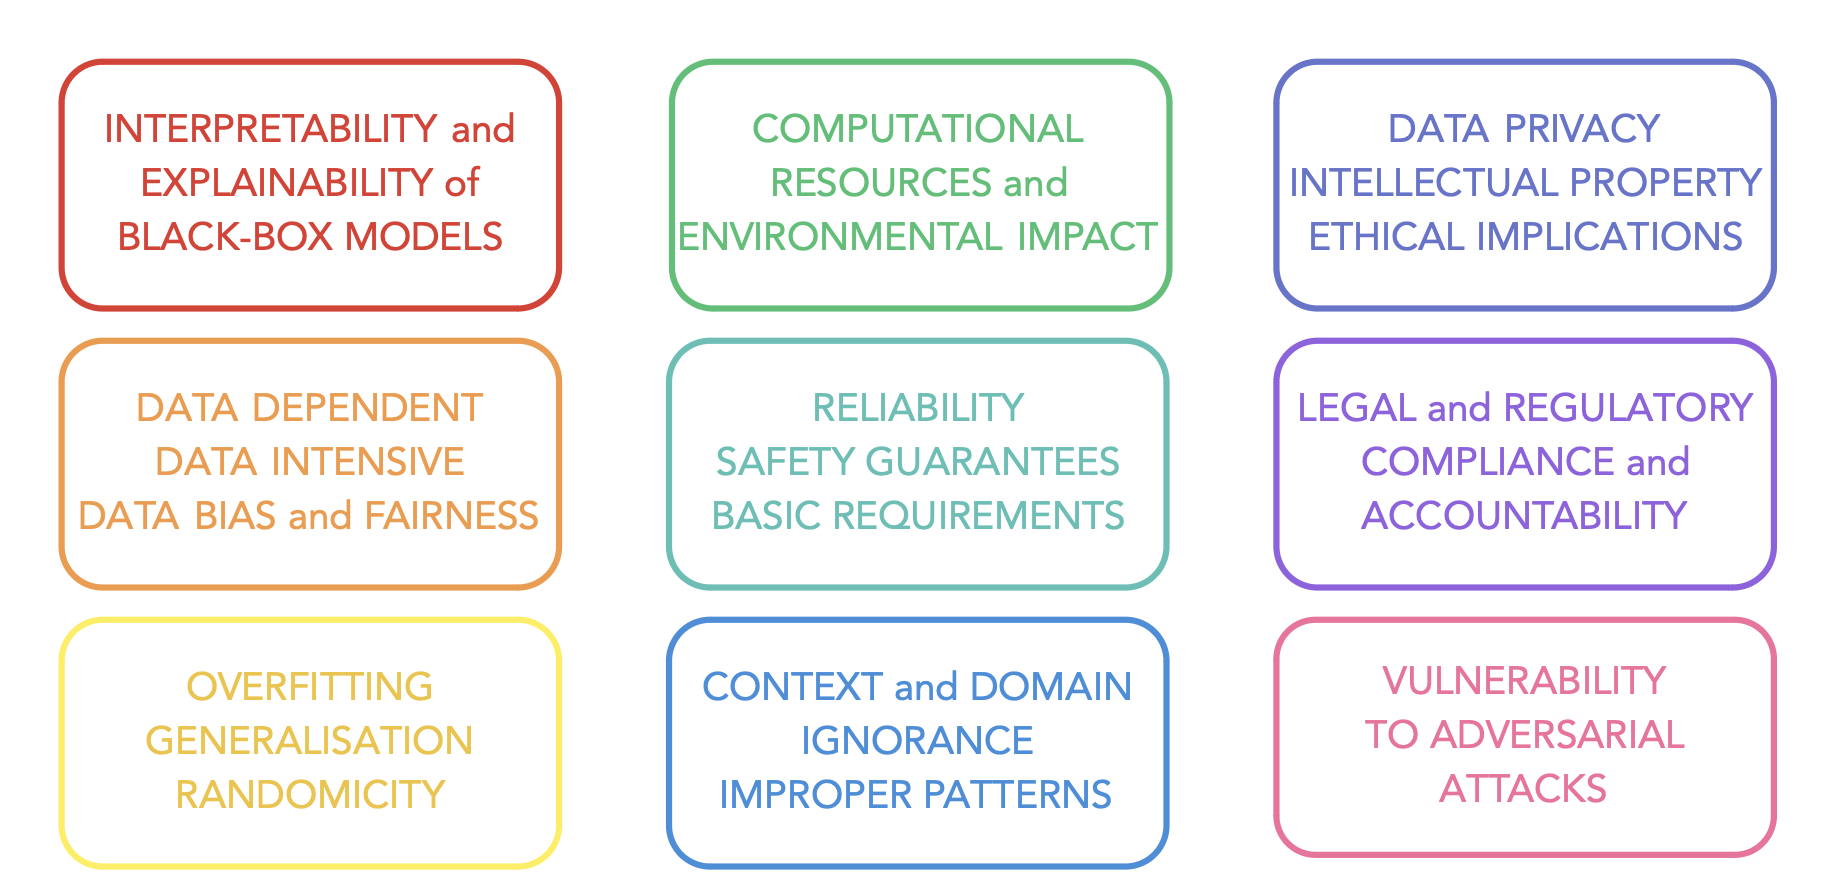
\includegraphics[width=0.65\textwidth]{imgs/MLProblems.png} 
 \end{figure} 
    
\centering{\alert{Still an open issue how to make them applicable to high-stakes or safety-critical application domains}}

\end{frame}


%\\\\\\\\\\\\\\\\\\\\\

\begin{frame}{Machine Learning in Medicine}

\begin{block}{Broad use of machine learning across different medical applications}

FDA: Graphical representation of the annual trends in FDA~\cite{joshi2024fda}

\begin{figure}
    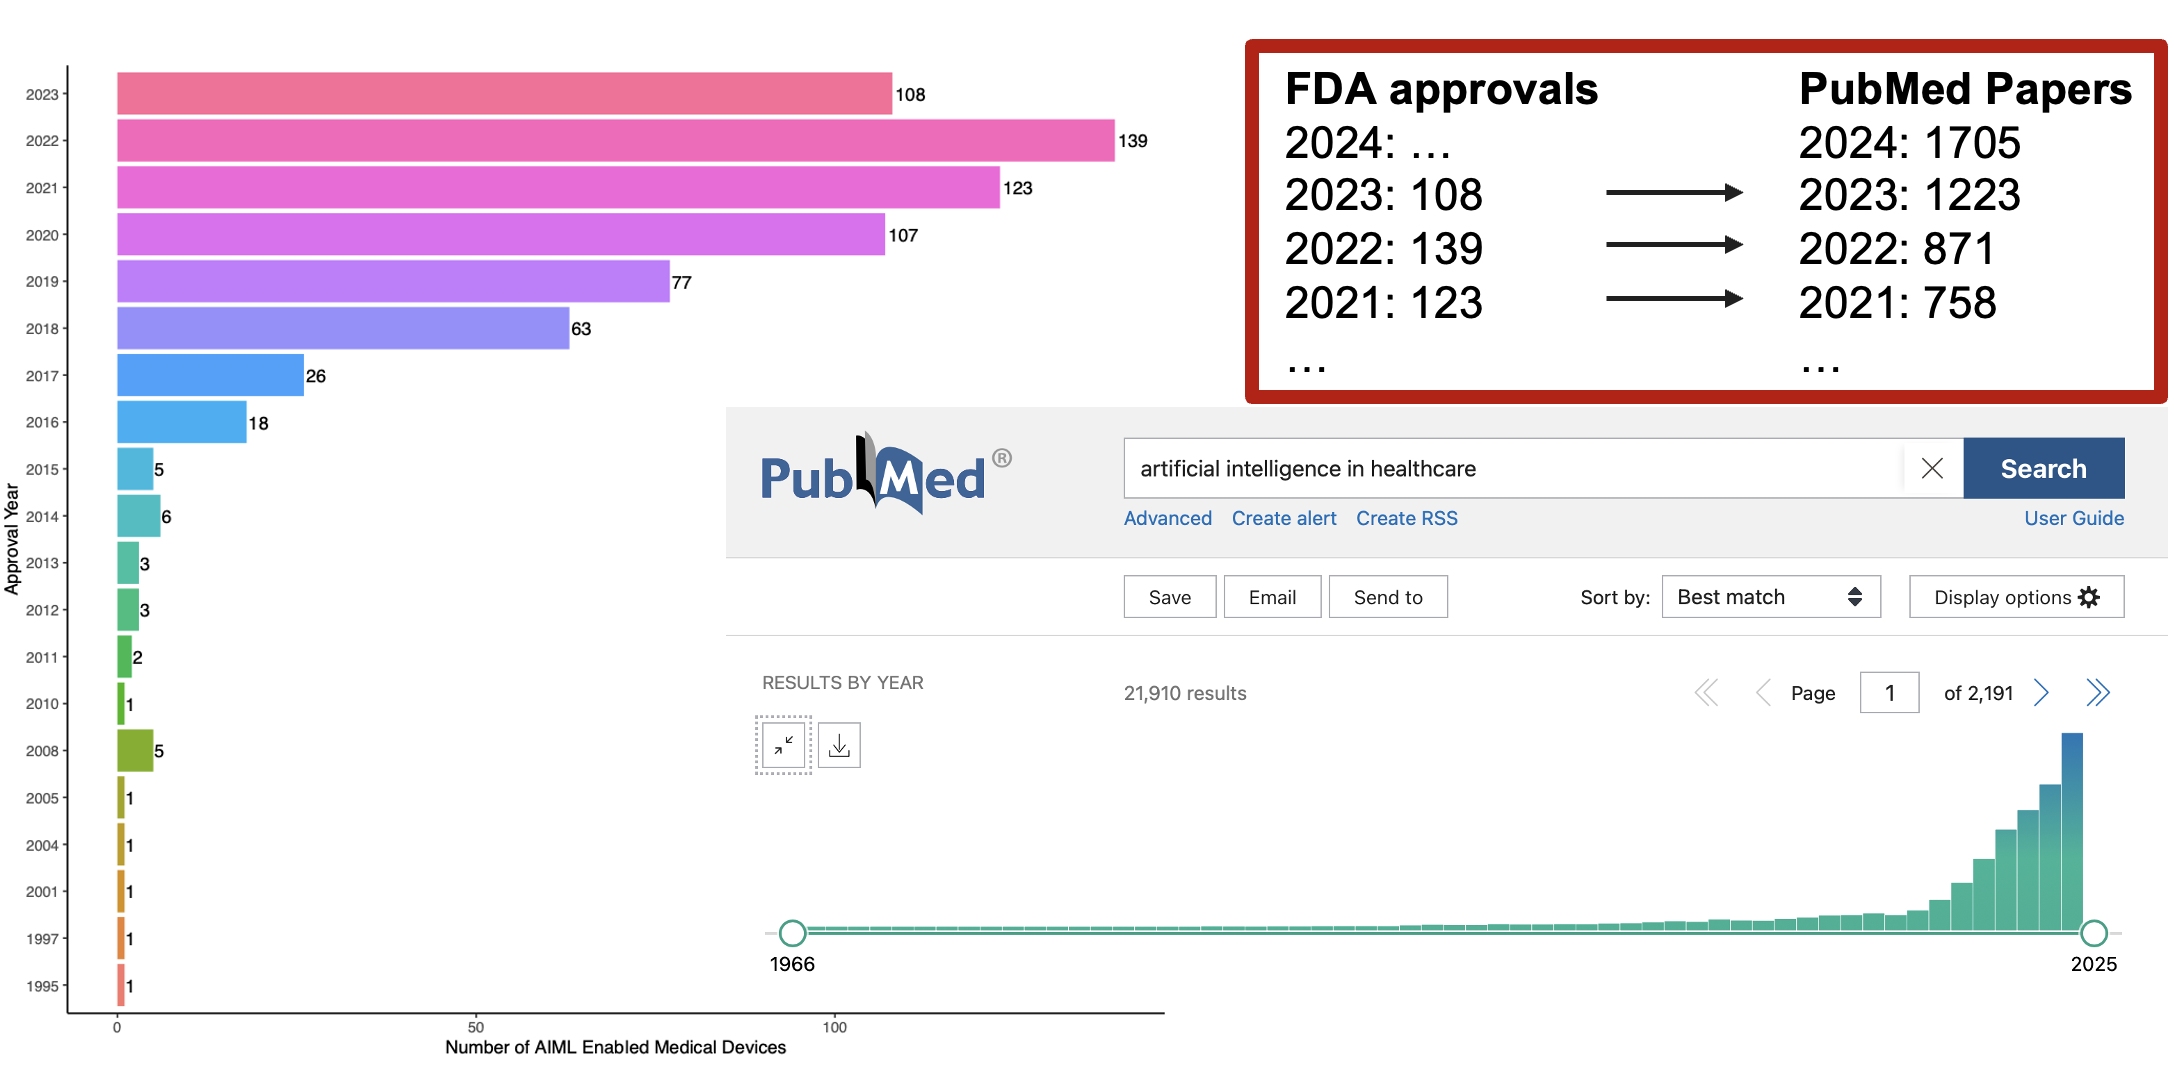
\includegraphics[width=0.8\textwidth]{imgs/FDA+papers.png} 
 \end{figure} 
 
 Despite numerous studies employing ML in medical data analysis, only a fraction have impacted clinical care
 
 \end{block}


 
 \tiny{[3] G. Joshi, A. Jain, S. R. Araveeti, S. Adhikari, H. Garg, and M. Bhandari, “Fda-approved artificial intelligence and machine learning (ai/ml)-enabled medical devices: An updated landscape,” Electronics, vol. 13, no. 3, p. 498, 2024[\href{http://creativecommons.org/licenses/by/4.0/}{CC BY 4.0}]}
\end{frame}
%%%%%%%%%%%%%%%%%%%%%%%%%%%%knowledge integration perché dovrebbe aiutare

\begin{frame}{Knowledge Integration into Data Driven Models}

\begin{block}{Goals}
    \begin{itemize}
        \item \textbf{Improve generalisation} Injecting prior knowledge into the model can guide learning, making it more robust to data sparsity, noise or overfitting
        \item \textbf{Reduce data dependency} Domain knowledge can help reduce the need for large labeled datasets, which are often expensive and time-consuming to gather
        \item \textbf{Incorporate interpretability} Knowledge integration can improve the transparency of the model, making it easier to explain decisions and ensuring trustworthiness
        \item \textbf{Enhance model efficiency} By constraining the learning process based on prior knowledge, models can converge faster and use fewer computational resources
    \end{itemize}
\end{block}

\end{frame}




%%%%%%%%%%%%%%%%%%%%%%

\begin{frame}{Informed Machine Learning Pipeline} 

{\centering{How prior knowledge can be integrated into the machine learning pipeline}}
\vspace{1em}

\begin{figure}
    \includegraphics[width=0.95\textwidth]{imgs/integration-pipeline.png} 
    \caption{Integration strategies~\cite{SirocchiBMC}  [\href{http://creativecommons.org/licenses/by/4.0/}{CC BY 4.0}]}
 \end{figure} 
 
 \vspace*{3em}
\tiny{[5] C. Sirocchi, A. Bogliolo, and S. Montagna, “Medical-informed machine learning: integrating prior knowledge into medical decision systems,” BMC Medical Informatics and Decision Making, vol. 24, no. 4, p. 186, 2024.}
 
\end{frame}



%%%%%%%%%%%%%%%%%%%%%%

\begin{frame}{Integration in Data Pre-Processing} 
\begin{figure}
    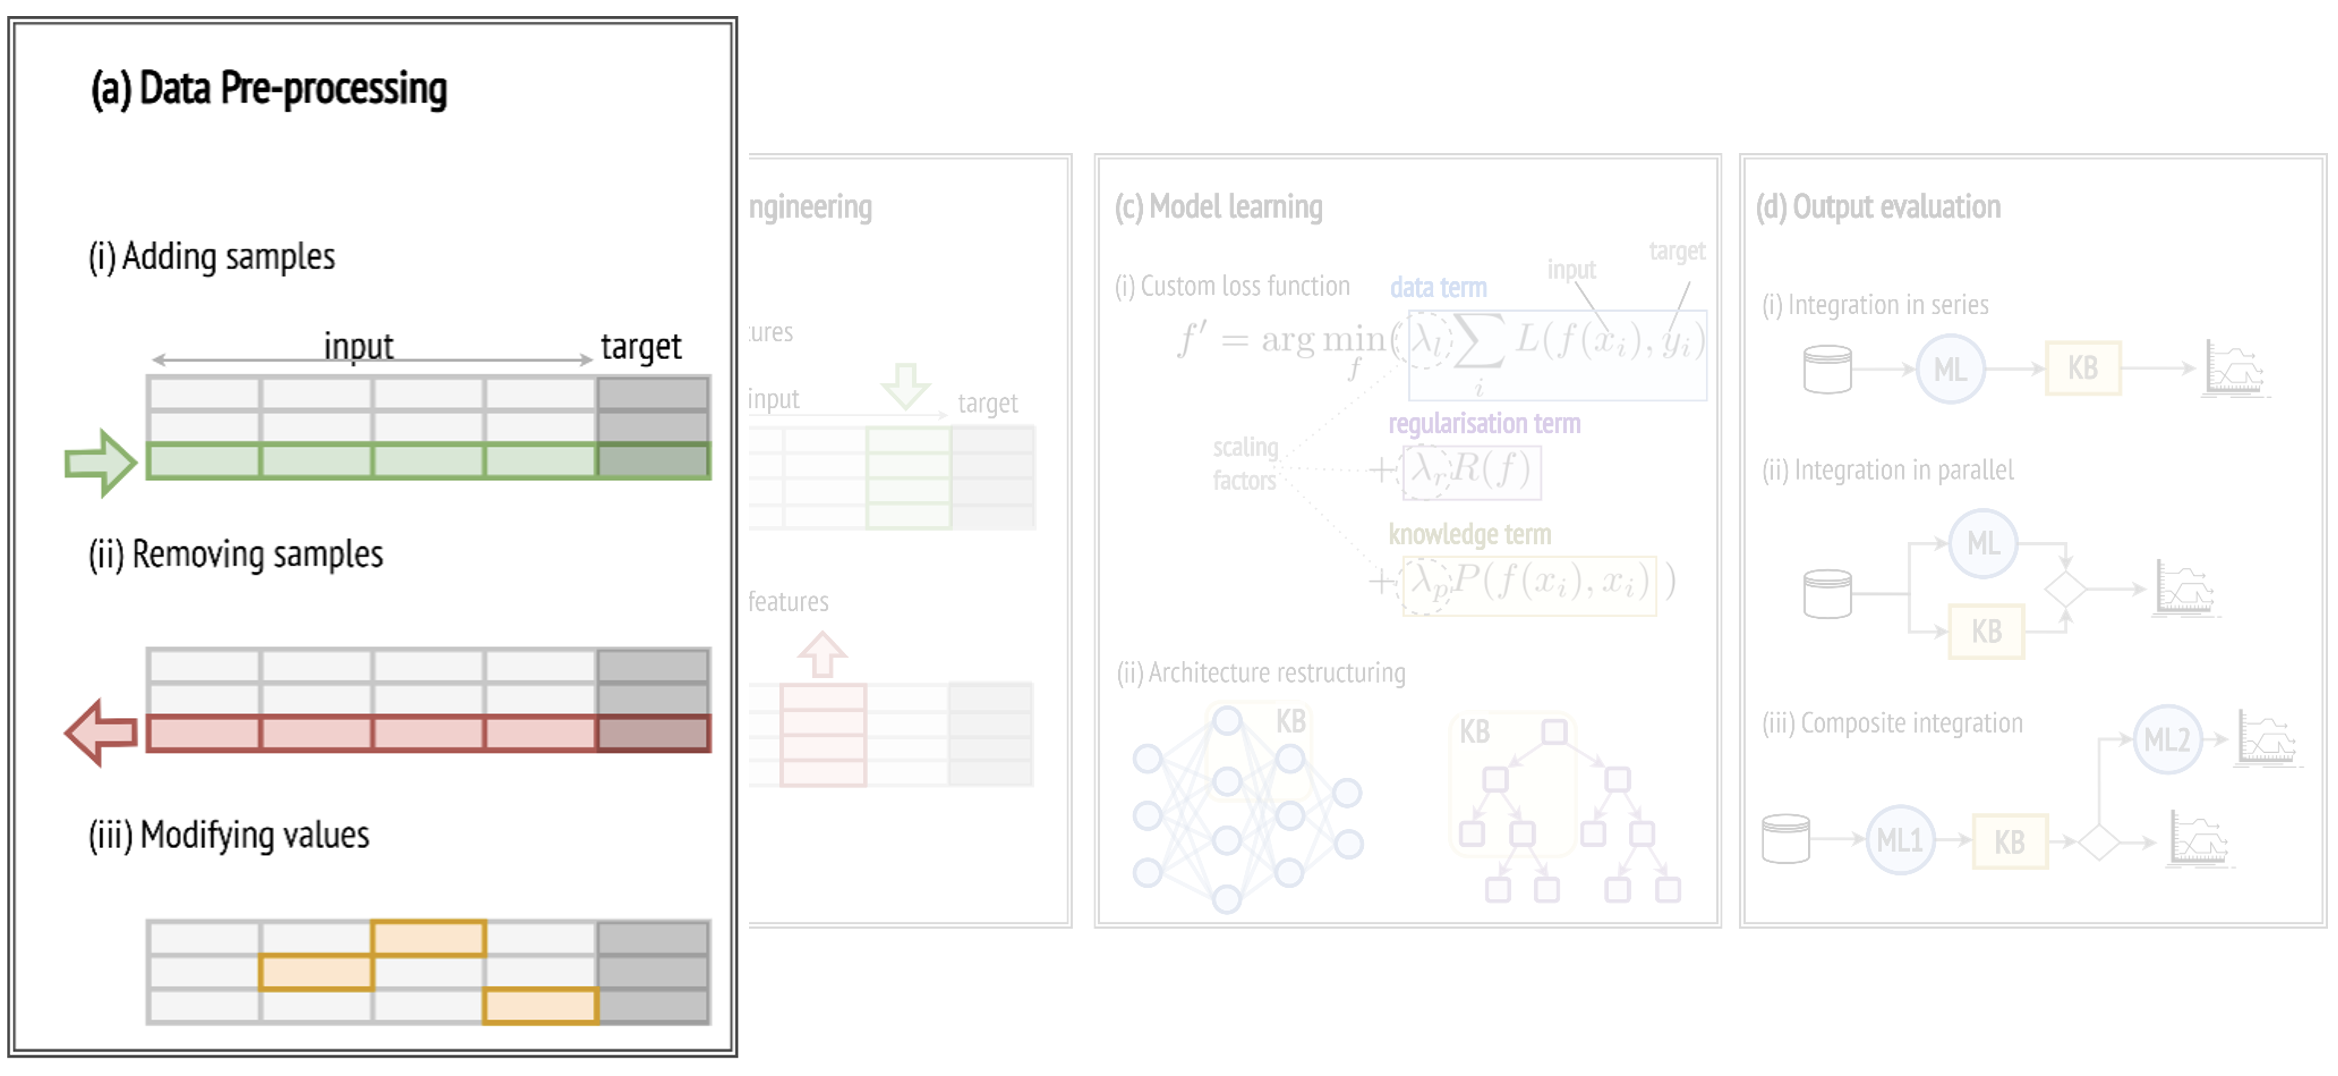
\includegraphics[width=0.9\textwidth]{imgs/integration-preprocessing.png} 
 \end{figure} 
 
\begin{block}{}
\begin{enumerate}
 	\item Data discretisation
 	\item Missing data imputation
	\item Data augmentation through simulation results
\end{enumerate}
\end{block}

\end{frame}

%%%%%%%%%%%%%%%%%%%%%%

\begin{frame}{Integration in Feature Engineering} 
\begin{figure}
    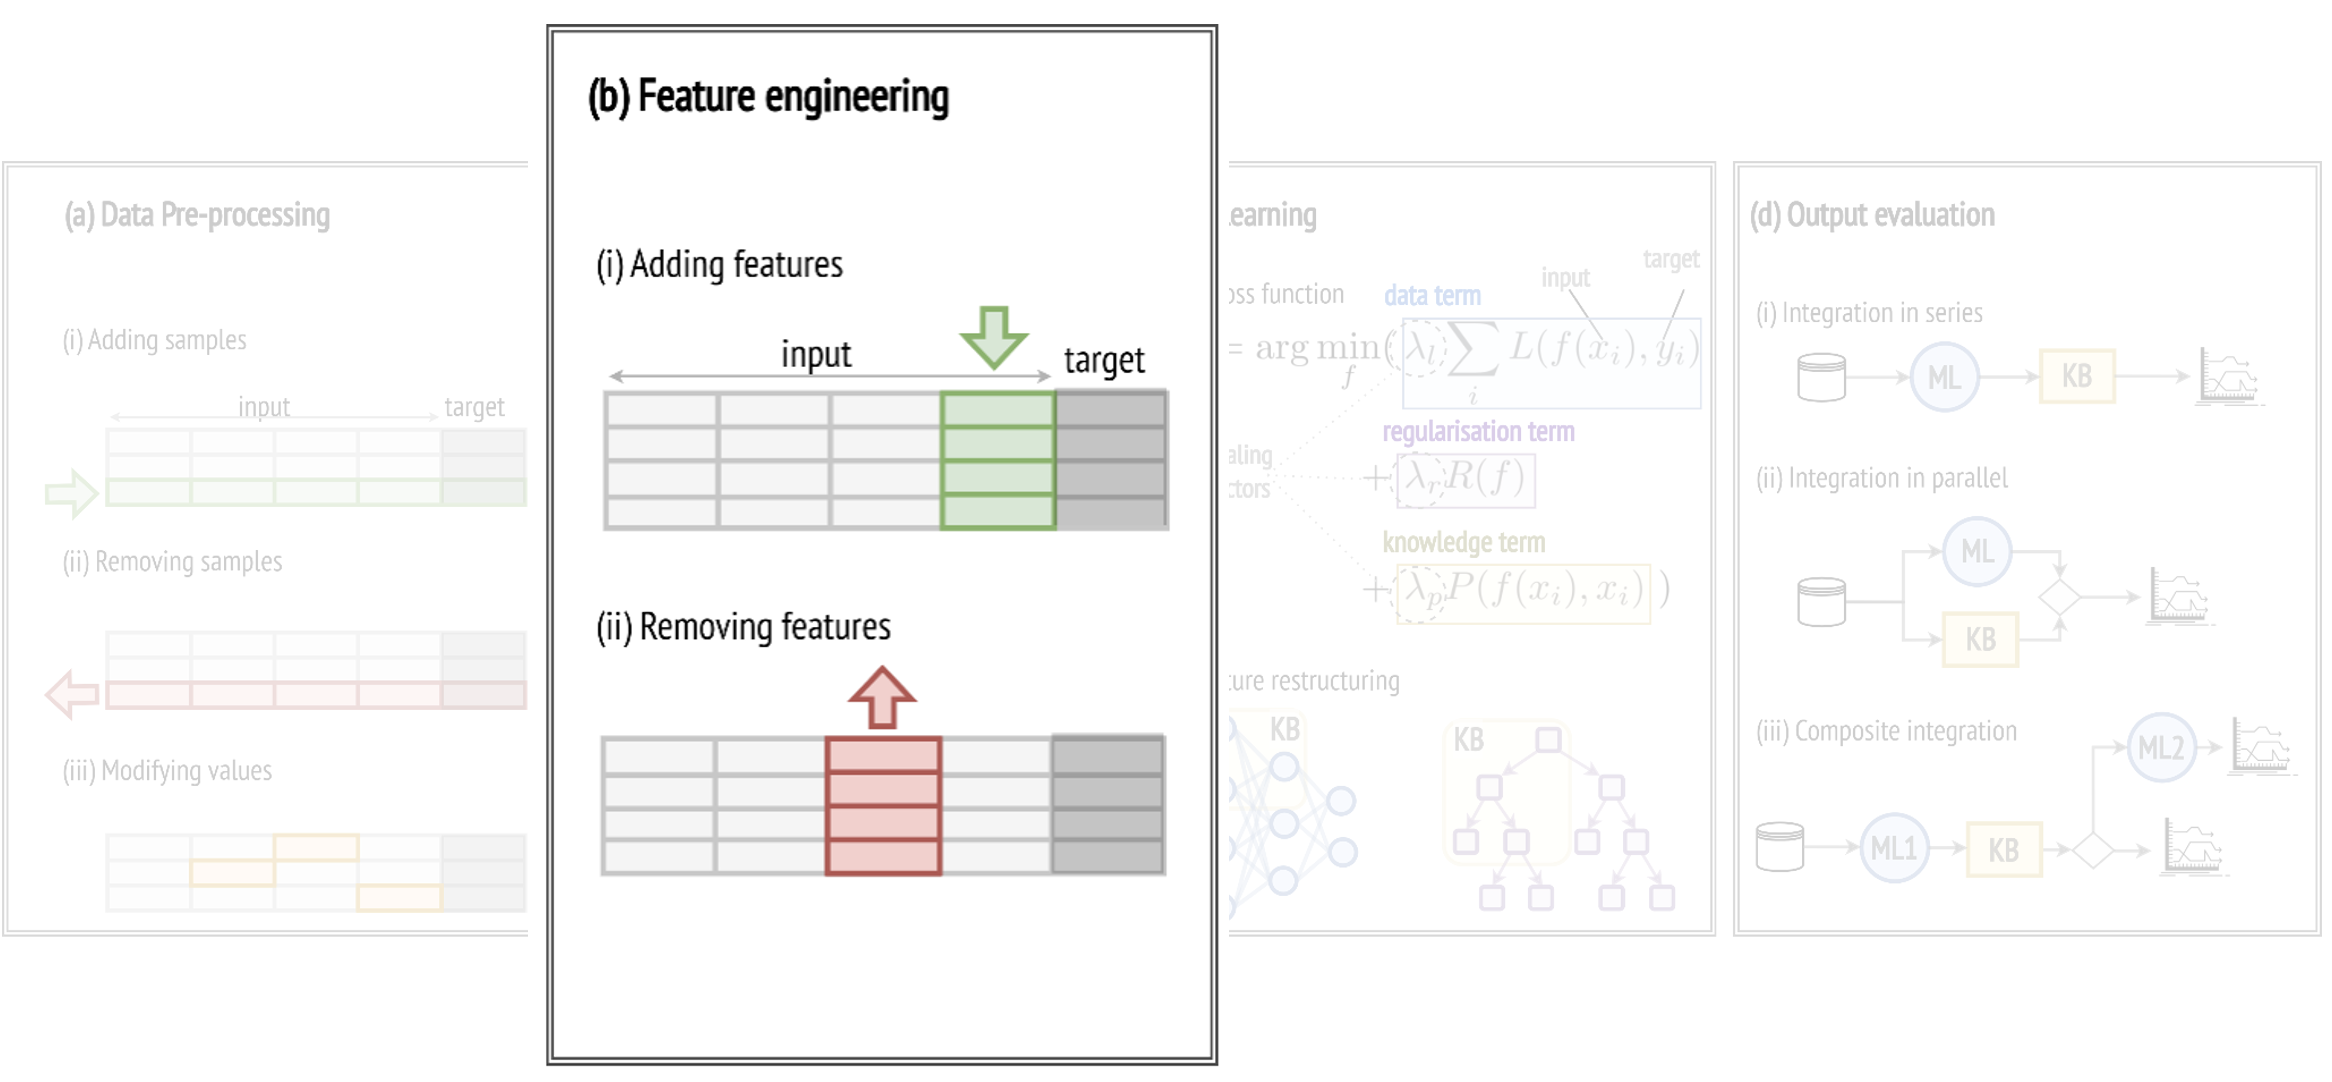
\includegraphics[width=0.9\textwidth]{imgs/integration-feateng.png} 
 \end{figure}  
 
\begin{block}{}
\begin{enumerate}
 	\item Derive additional features from existing ones using from the knowledge base
	\begin{itemize} 
		\item mathematical models 
		\item logical inference 
	\end{itemize}%. Combining several features into a few composite indices can reduce the dataset dimensionality while enhancing model accuracy and interpretability.
	\item Feature selection
\end{enumerate}
\end{block}

\end{frame}

%%%%%%%%%%%%%%%%%%%%%%

\begin{frame}{Integration in Model Learning} 
\begin{figure}
    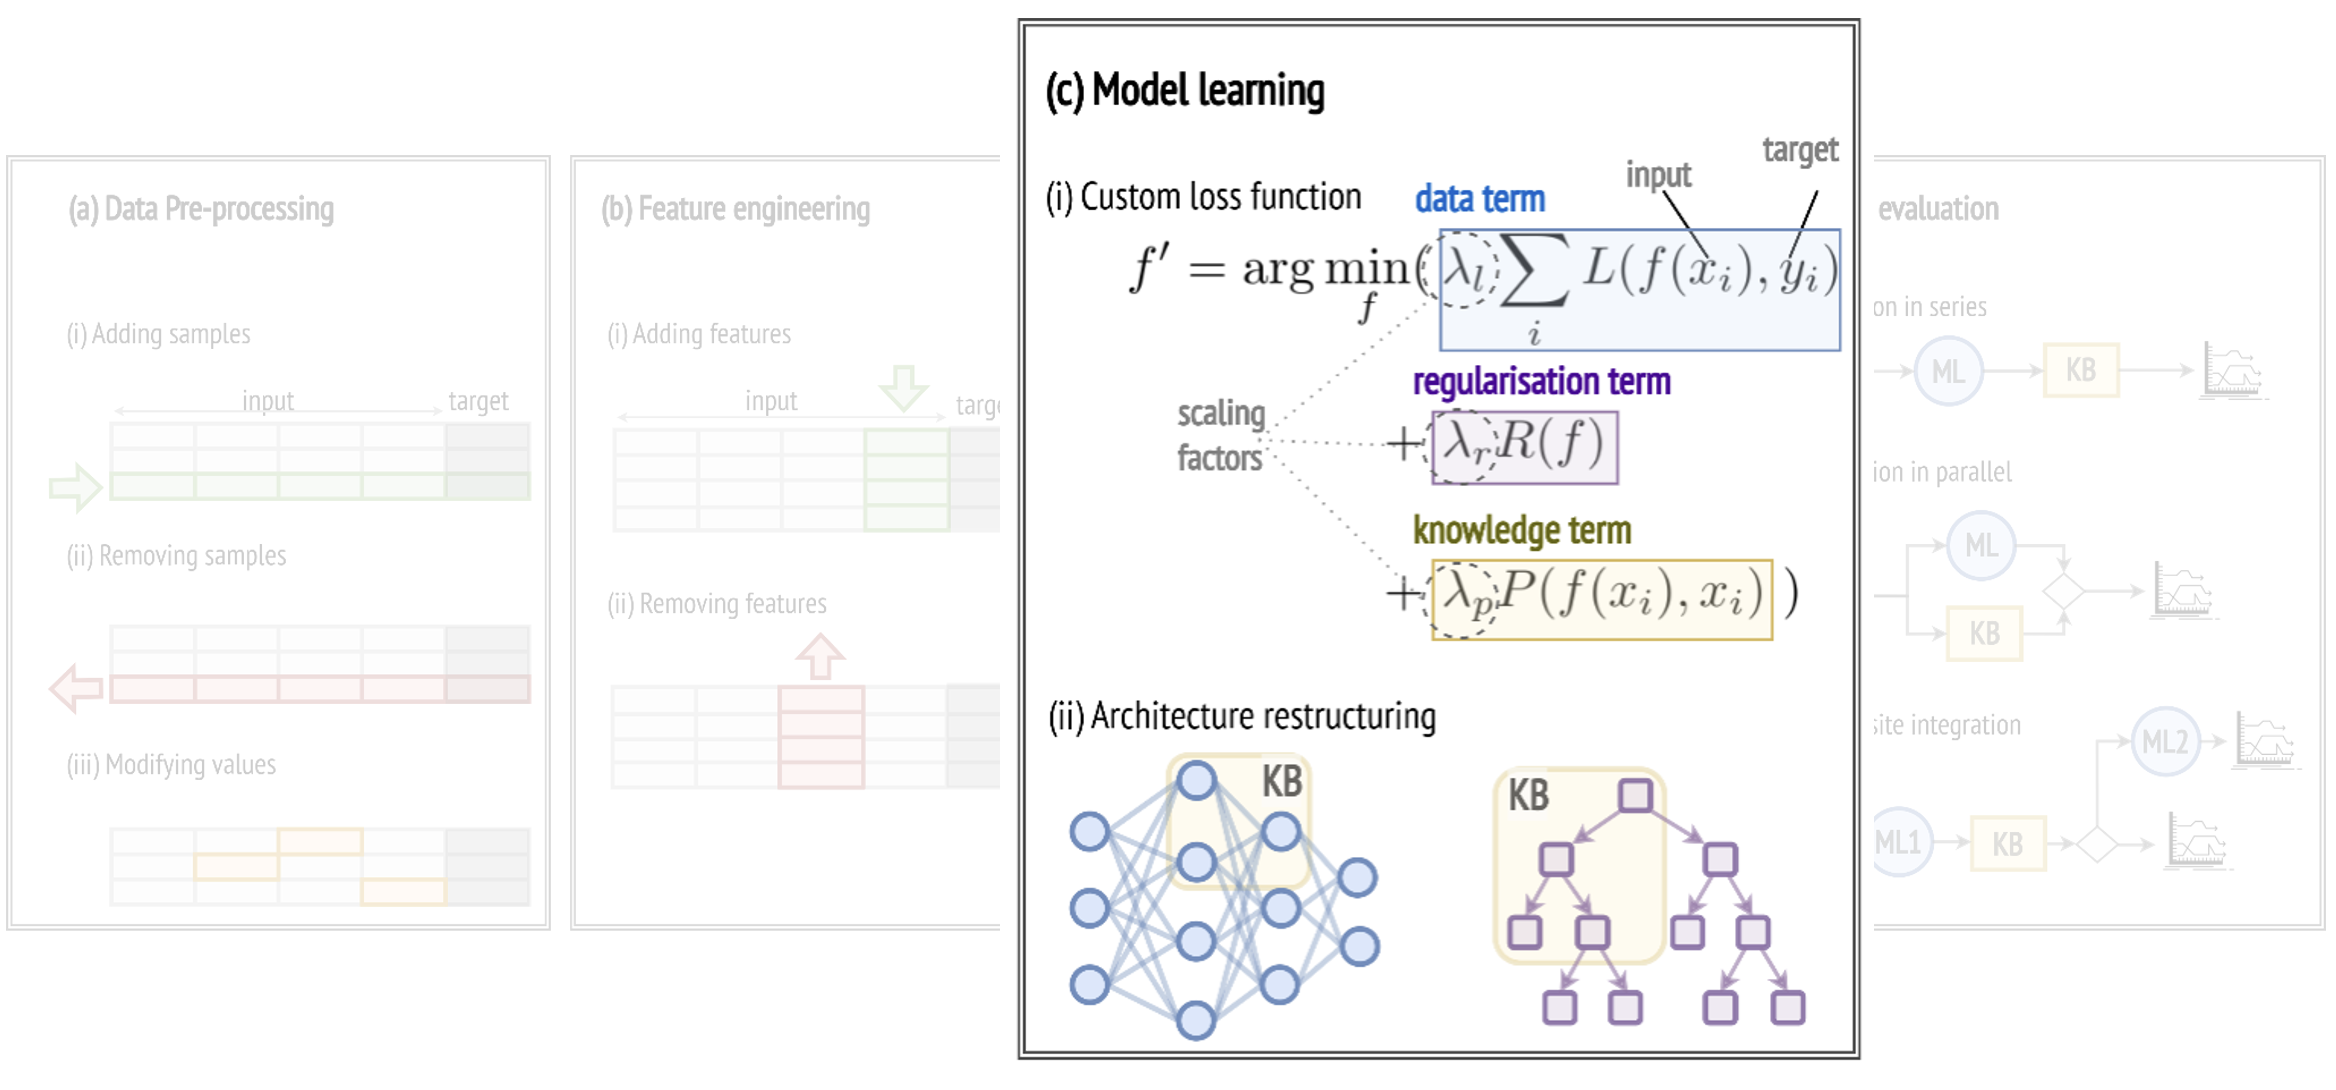
\includegraphics[width=0.9\textwidth]{imgs/integration-model-learning.png} 
 \end{figure} 
  
\begin{block}{}
\begin{enumerate}
 	\item Custom loss function: the  loss function that can be modified according to additional knowledge
 	\item Architecture restructuring: knowledge can be integrated by choosing model structure and hyper-parameters
\end{enumerate}
\end{block}

\end{frame}
%%%%%%%%%%%%%%%%%%%%%%

\begin{frame}{Integration in Output Evaluation} 
\begin{figure}
    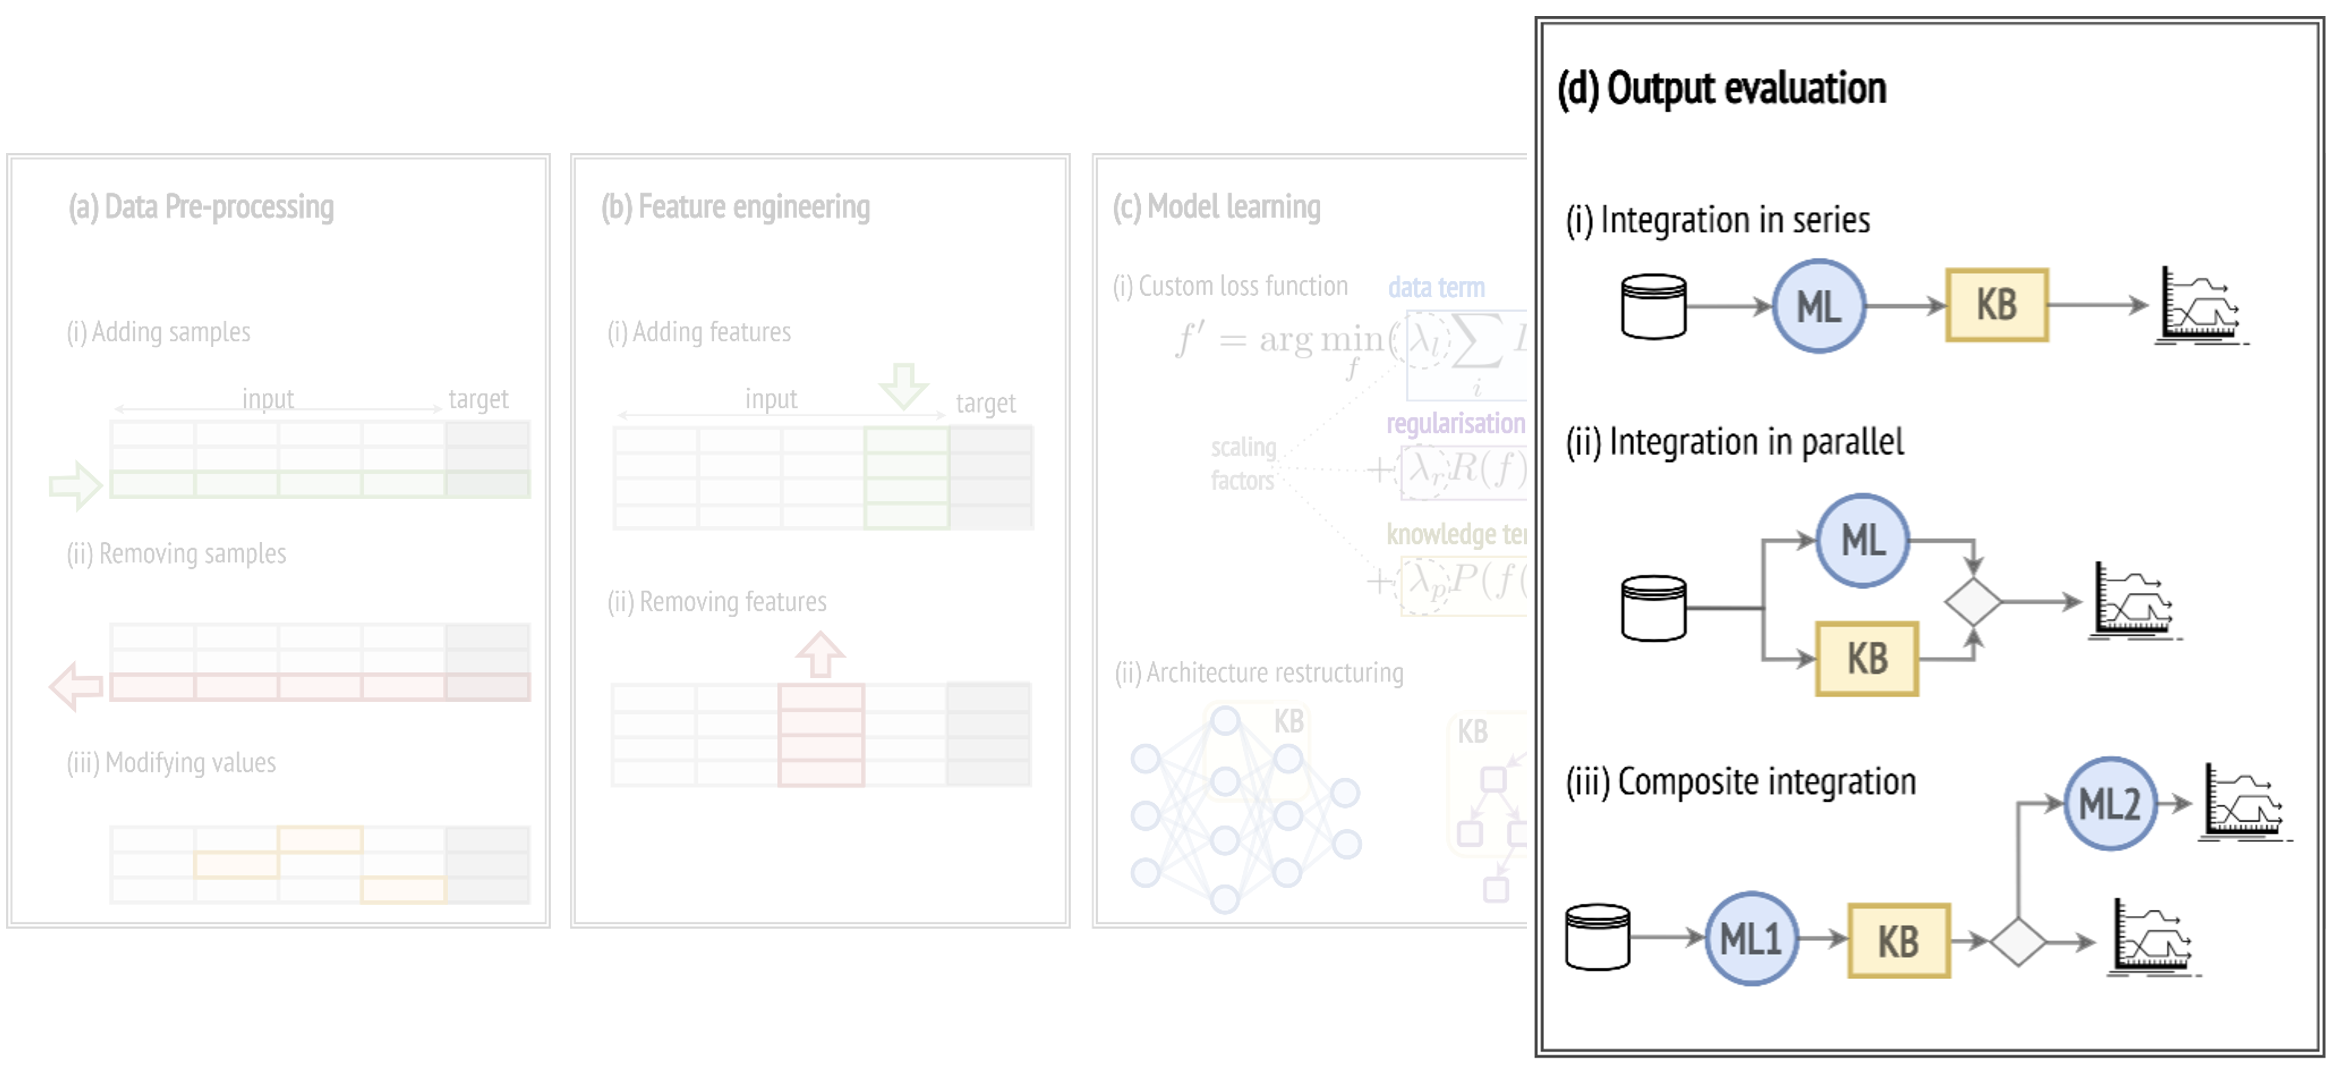
\includegraphics[width=0.9\textwidth]{imgs/integration-output-eval.png} 
 \end{figure} 
  
\begin{block}{}

The output of a learning pipeline can be combined or validated against existing knowledge:%. For example, predictions that do not agree with known constraints can be discarded or marked as suspicious so that results are consistent with prior knowledge.

\begin{enumerate}
 	\item Integration in series or in parallel
 	\item Composite integration
\end{enumerate}
\end{block}

\end{frame}

%%%%%%%%

\begin{frame}{Medical and Clinical Domain Knowledge Encoding}

\begin{figure}
    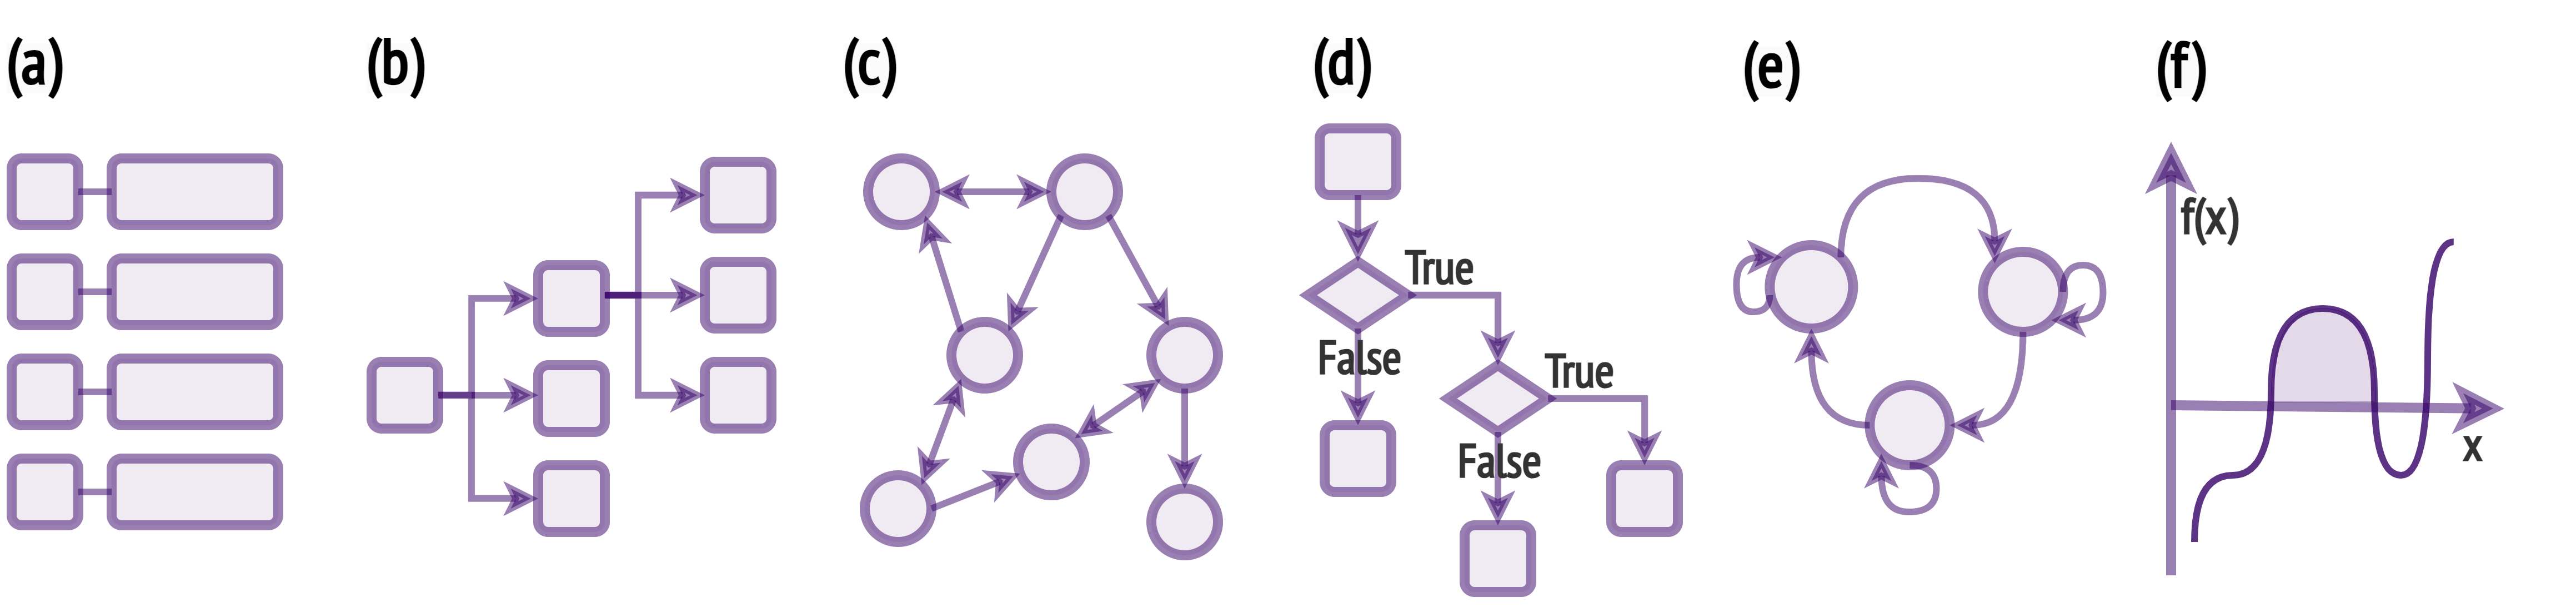
\includegraphics[width=0.9\textwidth]{imgs/knowledge_types.png} 
 \end{figure} 
 
 \begin{block}{(d) Focus on rules}
 \begin{itemize}
	\item Mirror clinical diagnostic reasoning and are often \alert{derived from standard clinical guidelines} or anatomical constraints 
	\item Rule-based decision support systems $\rightarrow$ \lbl{symbolic AI}
\end{itemize}
\end{block}



 \end{frame}
}
%%%%%%%%%%%%%%%%%%%%%%
\section[NeSy]{Neurosymbolic AI }
%%%%%%%%%%%%%%%%%%%%%%

%%%%%%%%%%%%%%%%%%%%%%
{
 \usebackgroundtemplate{}
 
%%%%%%%%%%%%%%%%%%%%%%

\begin{frame}{Neurosymbolic AI: where Symbolic Artificial Intelligence is Integrated in  Machine Learning}


\textbf{Neurosymbolic AI} refers to the integration of \textbf{Symbolic AI} with \textbf{Machine Learning (ML)} techniques, combining the strengths of both approaches

\begin{itemize}
    \item \textbf{Integration}: Neurosymbolic AI combines the interpretability and reasoning power of \alert{symbolic methods} with the \alert{data-driven} learning of ML models
    \item \textbf{Benefits}
        \begin{itemize}
            \item increase \alert{explainability} and \alert{trustability} of the system
	        	\item build a system that is \\\alert{rubust} to data \\degradation
        \end{itemize}
  
\end{itemize}
\vspace{-2.5em}
\begin{figure}
\hfill
    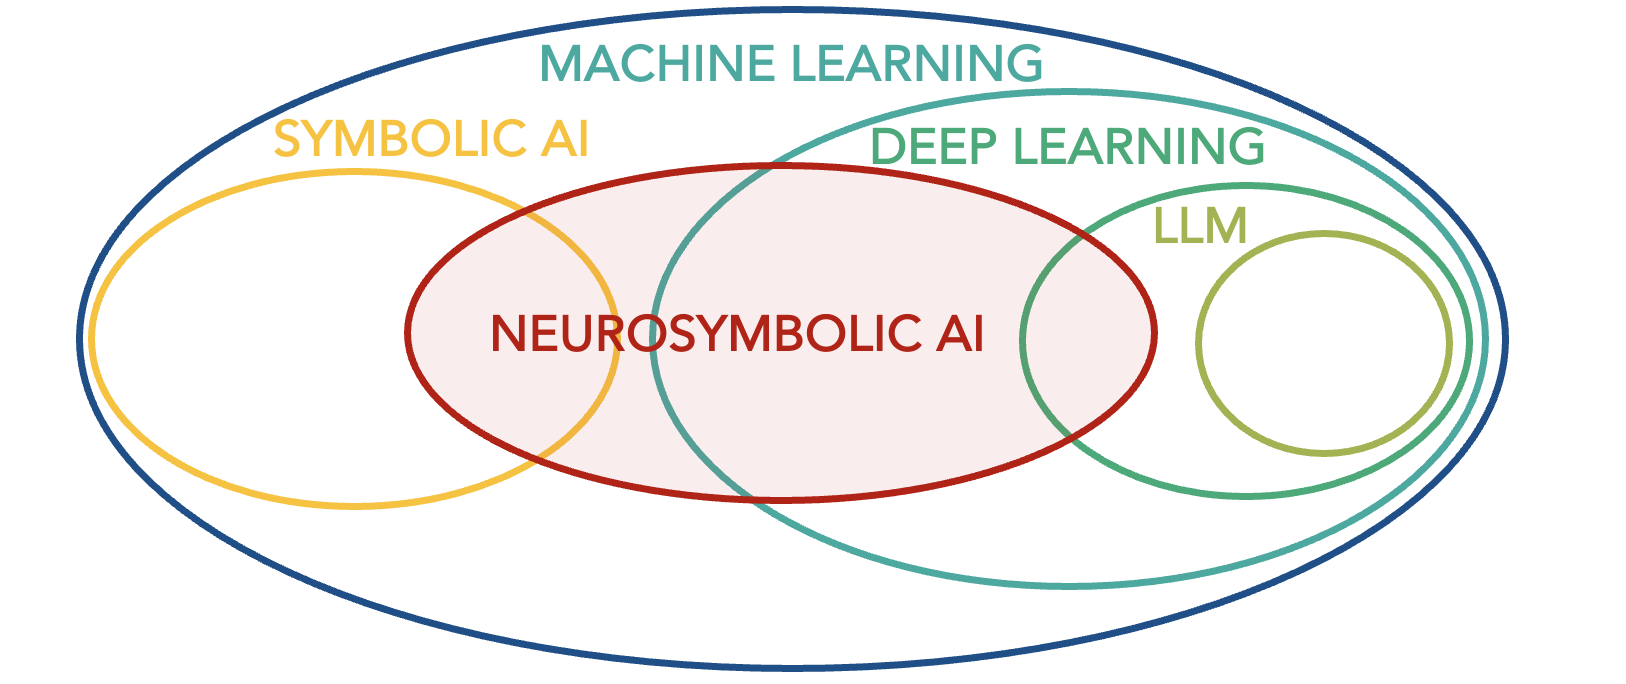
\includegraphics[width=0.65\textwidth]{imgs/neurosymb.png}
 \end{figure} 
 
\end{frame}



%%%%%%%%%%%%%%%%%%%%%%

\begin{frame}{The Framework of SKI}

\begin{figure}
    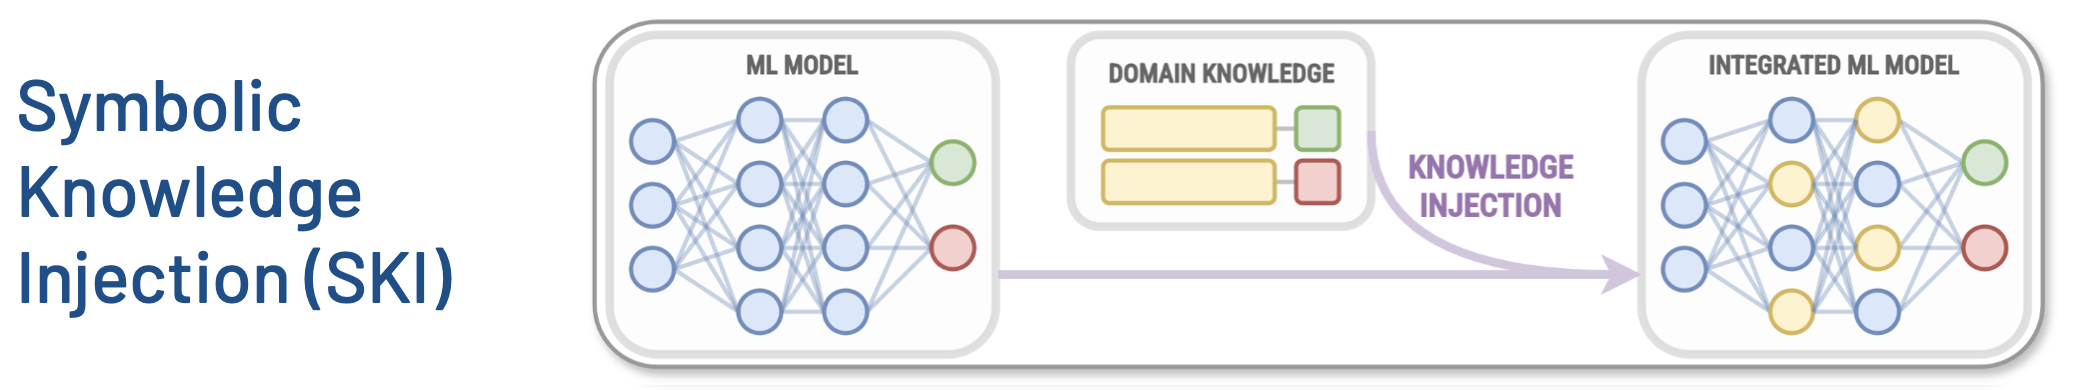
\includegraphics[width=0.95\textwidth]{imgs/SKI.png} 
 \end{figure} 
 \vfill
\begin{block}{SKI definition~\cite{skeislr-acmcs}}
Algorithms and procedures accepting symbolic knowledge as input and producing ML predictors as output \\
\alert{Uneducated $\rightarrow$ Educated model}
\end{block}

\vspace{2em}
\tiny{[2] G. Ciatto, F. Sabbatini, A. Agiollo, M. Magnini, and A. Omicini, “Symbolic knowledge extraction and injection with sub-symbolic predictors: A systematic literature review,” ACM Computing Surveys, vol. 56, no. 6, pp. 161:1–161:35, Jun. 2024.}

\end{frame}

%%%%%%%%%%%%%%%%%%%%%%

%\begin{frame}{SKI: How Symbolic Knowledge can be Integrated in ML}
%
%\begin{block}{We define SKI as~\cite{skeislr-acmcs}}
%
%\begin{quote}
%any algorithmic procedure affecting how sub-symbolic predictors draw their inferences in such a way that predictions are either computed as a function of, or made consistent with, some given symbolic knowledge.
%\end{quote}
%
%\end{block}
%
%\begin{itemize}
%
%	\item SKI algorithms are procedures accepting symbolic knowledge as input and producing ML predictors as output.
%	\item Knowledge should be symbolic and user provided ---hence, human interpretable
%	\item Since any input knowledge should be algorithmically manipulated by the SKI procedure, we elicit an implicit requirement here, constraining the input knowledge to be machine interpretable as well
%
%\end{itemize}
%\vspace{2em}
%\tiny{[2] G. Ciatto, F. Sabbatini, A. Agiollo, M. Magnini, and A. Omicini, “Symbolic knowledge extraction and injection with sub-symbolic predictors: A systematic literature review,” ACM Computing Surveys, vol. 56, no. 6, pp. 161:1–161:35, Jun. 2024.}
%
%\end{frame}




%\\\\\\\\\\\\\\\\\\\\\
\begin{frame}{Contribution of the Paper in Details}

\begin{block}{Explicitly state the contributions of the paper}
    \begin{enumerate}
  \item[RQ1] Is  SKI improving the \emph{performance} of  ML models?
  %
  In particular, recall and F1-score because of the medical domain's sensitivity to false negatives.
  %
  \item[RQ2] Is  SKI improving the \emph{adherence} of  ML models to established protocols?
  %
  Simply put, does the educated model make predictions more in line with the injected logic compared to the uneducated one?
  %
  \item[RQ3] Is  SKI improving the \emph{robustness} of  ML models in the presence of data degradation?
  %
  Does the performance of the educated predictor degrade less than that of the uneducated one when data are perturbed?
  %
%  \item[RQ4] Is  SKI} improving \emph{data efficiency}~(\cref{subsec:qos}) of  ML} models?
%  %
%  Equivalently, does the educated predictor achieve the same performance of the uneducated predictor with fewer data?
  %
\end{enumerate}
\end{block}

\end{frame}
%\\\\\\\\\\\\\\\\\\\\\
}
%===============================================================================
\section[Methods]{Model \& Metrics}
%===============================================================================
%%%%%%%%%%%%%%%%%%%%%%
{
 \usebackgroundtemplate{}
 
\begin{frame}{Logic Tensor Networks}
    Logic Tensor Networks (LTNs)~\cite{BadreddineGSS22} combine deep learning with symbolic reasoning, providing a framework for integrating logic and learning.
    Using a differentiable form of first-order logic called \textbf{Real Logic}, LTNs can:

    \begin{itemize}
        \item Learn from data and incorporate prior knowledge.
        \item Support logical reasoning during learning.
        \item Represent complex relationships using tensor representations.
    \end{itemize}

    \begin{figure}
        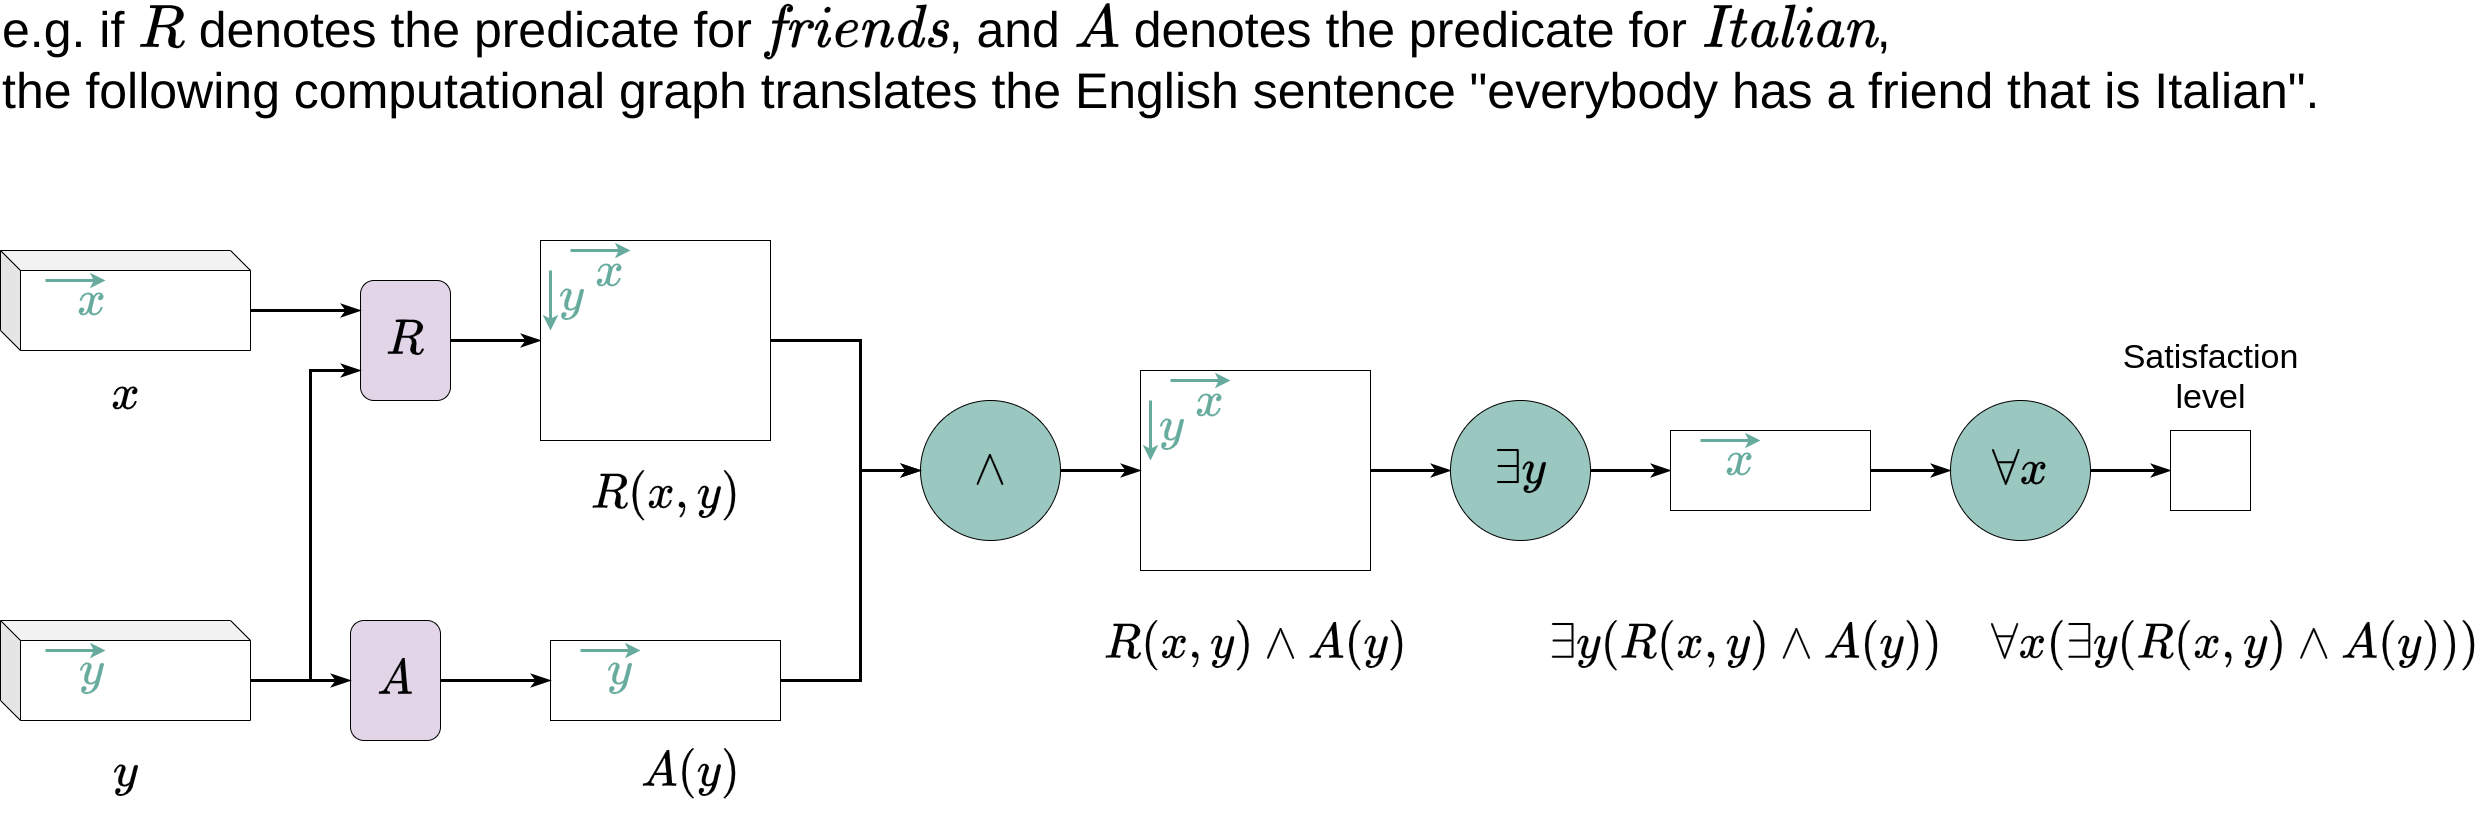
\includegraphics[width=0.9\textwidth]{figures/framework_computational_graph}
        \\
        \caption*{Source: \url{https://github.com/logictensornetworks/logictensornetworks}}
    \end{figure}

\end{frame}

%%%%%%%%%%%%%%%%%%%%%%%%%%%
\begin{frame}{Metrics}
    \begin{block}{Performance metrics}
    \begin{itemize}
	\item Used to evaluate the predictive capabilities of the  ML models
        \begin{itemize}
            \item Accuracy, Precision, Recall, F1-Score\ldots
        \end{itemize}
        \item They are the same for both the educated and uneducated models
         \end{itemize}
    \end{block}
    
    \begin{block}{Logic adherence}
       Metric to assess how well the model adheres to the clinical rules by comparing model predictions with logic formulas
    \end{block}
    
     \begin{block}{QOS -- Robustness to Data Degradation}
     \begin{itemize}
            \item Input data noisy, incomplete, or biased
            \item Data degradation may negatively affect the performance of a predictor, unless some  SKI procedure is in place to compensate for it
            \item The robustness of a predictor can be estimated by applying perturbations to the training data and assessing performance on the perturbed data
            \end{itemize}
%            A robustness score can be computed as:
%        
%        \[
%            \rho_{N, D}(\mathbf{D}) = \frac{1}{n} \sum_{\Delta D \in \mathbf{D}} \left\lVert \Delta D \right\rVert \cdot \frac{\pi(N_{\Delta D}, D \circ \Delta D)}{\pi(N, D)}
%        \]
    \end{block}
    
\end{frame}





}\label{sec:theory-/-modelling-/-design}
%\\\\\\\\\\\\\\\\\\\\\

\section[Case Study]{Case study: Experiments \& Results}
%%%%%%%%%%%%%%%%%%%%%%
{
 \usebackgroundtemplate{}
 
%\\\\\\\\\\\\\\\\\\\\\
\begin{frame}{Diabetes Risk Prediction}

\begin{block}{Knowledge base for predicting risk of type-2 diabetes as formalised in~\cite{kunapuli2010online}.}
\begin{table}[!h]

\label{tab:rules}
%\raggedright
%\renewcommand{\arraystretch}{1.5}
\begin{tabular}{|lll|}
\hline
Rule 1 & & $(BMI \geq 30) \land (G_{120} \geq 126) \implies \text{diabetes}$ \\
Rule 2 & & $(BMI \leq 25) \land (G_{120} \leq 100) \implies \text{healthy}$ \\
\hline
\end{tabular}
\end{table}
\end{block}

The dataset comprises 768 medical profiles of women aged $\geq$ 21. \\ The target variable is binary, indicating a diabetes diagnosis within five years. 


\begin{block}{Pima Indians Diabetes dataset}
\begin{table}[h]
\scriptsize{
\begin{tabular}{@{}lcl@{}}
\toprule
Feature name & Code & Description\\ 
\midrule
Pregnancies & & Number of times pregnant\\
Glucose & $G_{120}$ & 2-hour plasma glucose concentration \\
Blood Pressure & $BP$ & Diastolic blood pressure\\
Skin Thickness & $ST$ & Triceps skin-fold thickness\\
Insulin & $I_{120}$ & 2-hour serum insulin \\
Body mass index & $BMI$ & Body mass index as weight/(height)$^2$ \\
Diabetes Pedigree Function & $DPF$ & Likelihood function of diabetes \\
	 &  &  based on family history~\cite{smith1988using}\\
Age & & Age in years\\
\midrule
\end{tabular}
}

\label{tab:pima}%
\end{table}
\end{block}

\end{frame}


%\\\\\\\\\\\\\\\\\\\\\
\begin{frame}{Trained Models and Hyperparameters}

\begin{block}{Reference models' hyperparameters}
%
\begin{description}
  \item[KNN] with $k=7$ and $L1$ distance;
  \item[DT] with entropy as split criterion and maximum depth of 10;
  \item[RF] with 50 trees, maximum depth of 20, entropy as criterion, and minimum number of samples per leaf of 5;
  \item[LR] with a regularisation parameter of 10, a maximum number of iterations of 1000 and liblinear as the solver.
\end{description}
\end{block}


\begin{block}{MLP (uneducated) and LTN (educated)}
Feedforward NN with the following architecture:
%
\begin{itemize}
  \item Input layer with 8 neurones, one for each feature in the dataset, LeakyReLU as activation function and batch normalisation;
  \item First, second and third hidden layer with respectively 256, 128, and 64 neurones, using LeakyReLU and batch normalisation;
  \item Output layer with 1 neurone and sigmoid function.
\end{itemize}
\end{block}

\end{frame}


%\\\\\\\\\\\\\\\\\\\\\
\begin{frame}

\begin{block}{\textbf{RQ1} -- Is SKI improving the \emph{performance}?}
\begin{table}[]
\centering
\begin{adjustbox}{max width=\textwidth}
\begin{tabular}{|l|c|c|c|c|c|c|}
\hline
\textbf{Model} & \textbf{Accuracy} & \textbf{Precision} & \textbf{Recall} & \textbf{F1 Score} & \textbf{Balanced Accuracy} & \textbf{MCC} \\
\hline
KNN                  & 0.738 $\pm$  0.02 & 0.636 $\pm$  0.03 & 0.583 $\pm$  0.05 & 0.607 $\pm$  0.03 & 0.702 $\pm$  0.02 & 0.413 $\pm$  0.05 \\
\hline
Decision Tree        & 0.697 $\pm$  0.02 & 0.565 $\pm$  0.03 & 0.580 $\pm$  0.05 & 0.571 $\pm$  0.03 & 0.670 $\pm$  0.02 & 0.339 $\pm$  0.05 \\
\hline
Random Forest        & 0.758 $\pm$  0.02 & 0.677 $\pm$  0.03 & 0.592 $\pm$  0.05 & 0.630 $\pm$  0.03 & 0.720 $\pm$  0.02 & 0.456 $\pm$  0.04 \\
\hline
Logistic Regression  & \textbf{0.763 $\pm$  0.02 }& \textbf{0.702 $\pm$  0.04} & 0.560 $\pm$  0.04 & 0.622 $\pm$  0.03 & 0.716 $\pm$  0.02 & 0.460 $\pm$  0.04 \\
\hline
MLP                  & 0.754 $\pm$  0.02 & 0.644 $\pm$  0.03 & 0.665 $\pm$  0.05 & 0.653 $\pm$  0.03 & 0.733 $\pm$  0.02 & 0.464 $\pm$  0.04 \\
\hline
Logic Tensor Network & 0.747 $\pm$  0.02 & 0.620 $\pm$  0.03 & \textbf{0.725 $\pm$  0.05} & \textbf{0.666 $\pm$  0.02} & \textbf{0.742 $\pm$  0.02} & \textbf{0.471 $\pm$  0.03} \\
\hline
\end{tabular}
\end{adjustbox}
\vspace{0.5em}
\caption{
  Performance Metrics (Mean $\pm$  Std) for Models.
  %
  The best scores are highlighted in bold.
  %
  According to the Wilcoxon signed-rank test with p-value=0.05, the LTN model outperforms all other models in terms of Recall, F1 Score, and Balanced Accuracy.
}
\label{tab:performance}
\end{table}
\end{block}

\begin{block}{\textbf{RQ2} -- Is SKI improving the \emph{adherence}?}
\begin{table}[]
  \centering
  {\fontsize{8}{12}\selectfont
  \begin{adjustbox}{max width=\textwidth}
    \begin{tabular}{|l|c|c|}
      \hline
      \textbf{Model} & \textbf{Rule 1} & \textbf{Rule 2} \\
      \hline
      KNN                   & 70.8 $\pm$  4.8   & 100.0 $\pm$  0.0 \\
      \hline
      Decision Tree         & 66.5 $\pm$  6.3   & 97.0 $\pm$  4.8 \\
      \hline
      Random Forest         & 76.6 $\pm$  5.1   & 100.0 $\pm$  0.0 \\
      \hline
      Logistic Regression   & 75.0 $\pm$  4.2   & 100.0 $\pm$  0.0 \\
      \hline
      MLP                  & 82.0 $\pm$  5.8   & 100.0 $\pm$  0.0 \\
      \hline
      Logic Tensor Network  & \textbf{87.4 $\pm$  5.2 }  & 100.0 $\pm$  0.0 \\
      \hline
    \end{tabular}
  \end{adjustbox}}
  \vspace{0.5em}
  \caption{Logic Adherence: Results for Rule 1 and Rule 2 (Mean $\pm$  Std) across Various Models}\label{tab:logic}

\end{table}

\end{block}

\end{frame}

%\\\\\\\\\\\\\\\\\\\\\

\begin{frame}{}
\begin{block}{\textbf{RQ3} -- Is SKI improving the \emph{robustness}?}
\begin{figure}
\begin{center}
	 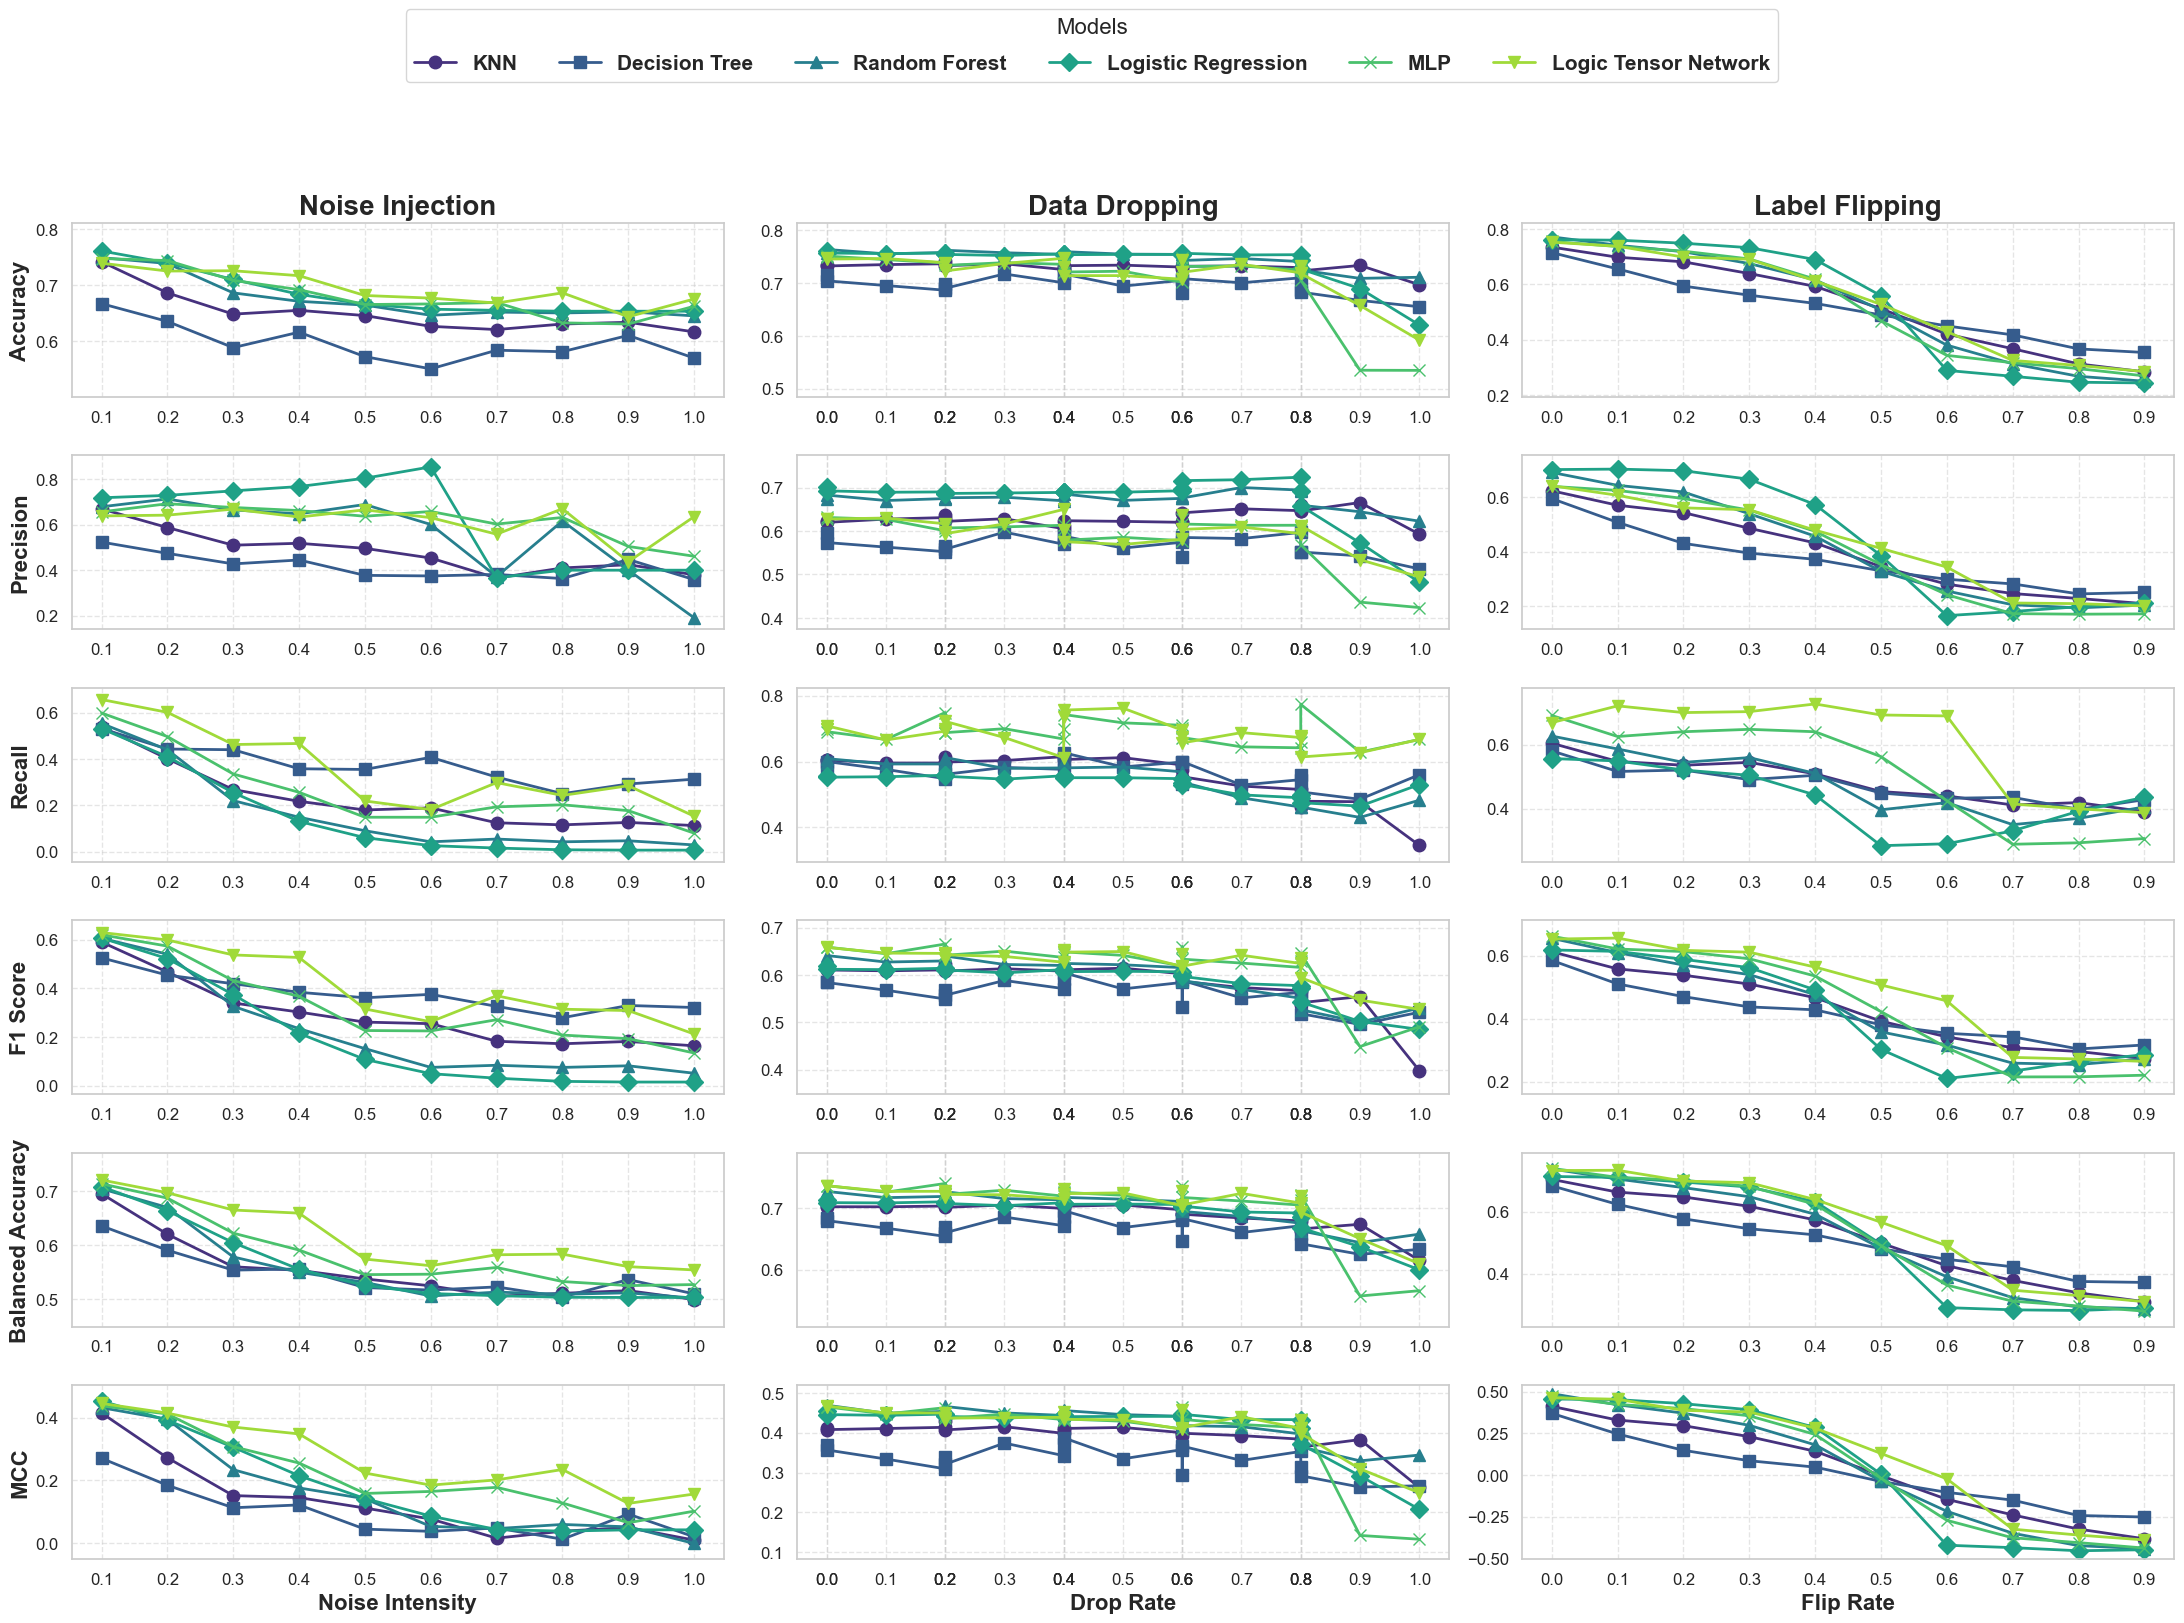
\includegraphics[width=0.75\textwidth]{imgs/improved_robustness_plot}
\caption{Model robustness under three common clinical data perturbations: noise injection from faulty devices, data loss from missing records, and label flipping due to incorrect diagnoses.}
\label{fig:robustness}
\end{center}
\end{figure}
\end{block}
\end{frame}

%\\\\\\\\\\\\\\\\\\\\\
}
\section[Discussion]{Conclusions \& Future Works}
{
 \usebackgroundtemplate{}

\begin{frame}
\frametitle{Conclusions \& Future Works}

\begin{block}{Summing up}
\begin{itemize}
\item LTN outperforms classical ML models in \emph{recall}, as a clinically relevant metrics
\item Injecting domain knowledge ensures \emph{adherence} to logic
\item LTN is \emph{robust} to data perturbations, demonstrating strong resilience
\end{itemize}
\end{block}

\begin{exampleblock}{Future works}
\begin{itemize}
\item Explore other SKI  methods and their computational complexity
\item Investigate the potential of smaller, knowledge-injected models in improving explainability and efficiency of uneducated larger models
\item Test over different datasets
\end{itemize}
\end{exampleblock}

\end{frame}



%\\\\\\\\\\\\\\\\\\\\\
%\begin{frame}%[allowframebreaks]
%\frametitle{Conclusions \& future works}
%
%\begin{block}{Summing up}
%    Summarise the most relevant contributions of this study:
%    %
%    \begin{itemize}
%        \item conclusion 1
%        \item conclusion 2
%        \item conclusion 3
%    \end{itemize}
%\end{block}
%
%\begin{exampleblock}{Future works}
%    Sketch some future research directions
%    %
%    \begin{itemize}
%        \item future work 1
%        \item future work 2
%    \end{itemize}
%\end{exampleblock}
%
%(may be split into 2 slides)
%
%\end{frame}
%\\\\\\\\\\\\\\\\\\\\\

\begin{frame}{Conclusions}
\centering{\Large{Thank you!}}
\vfill
\begin{figure}
    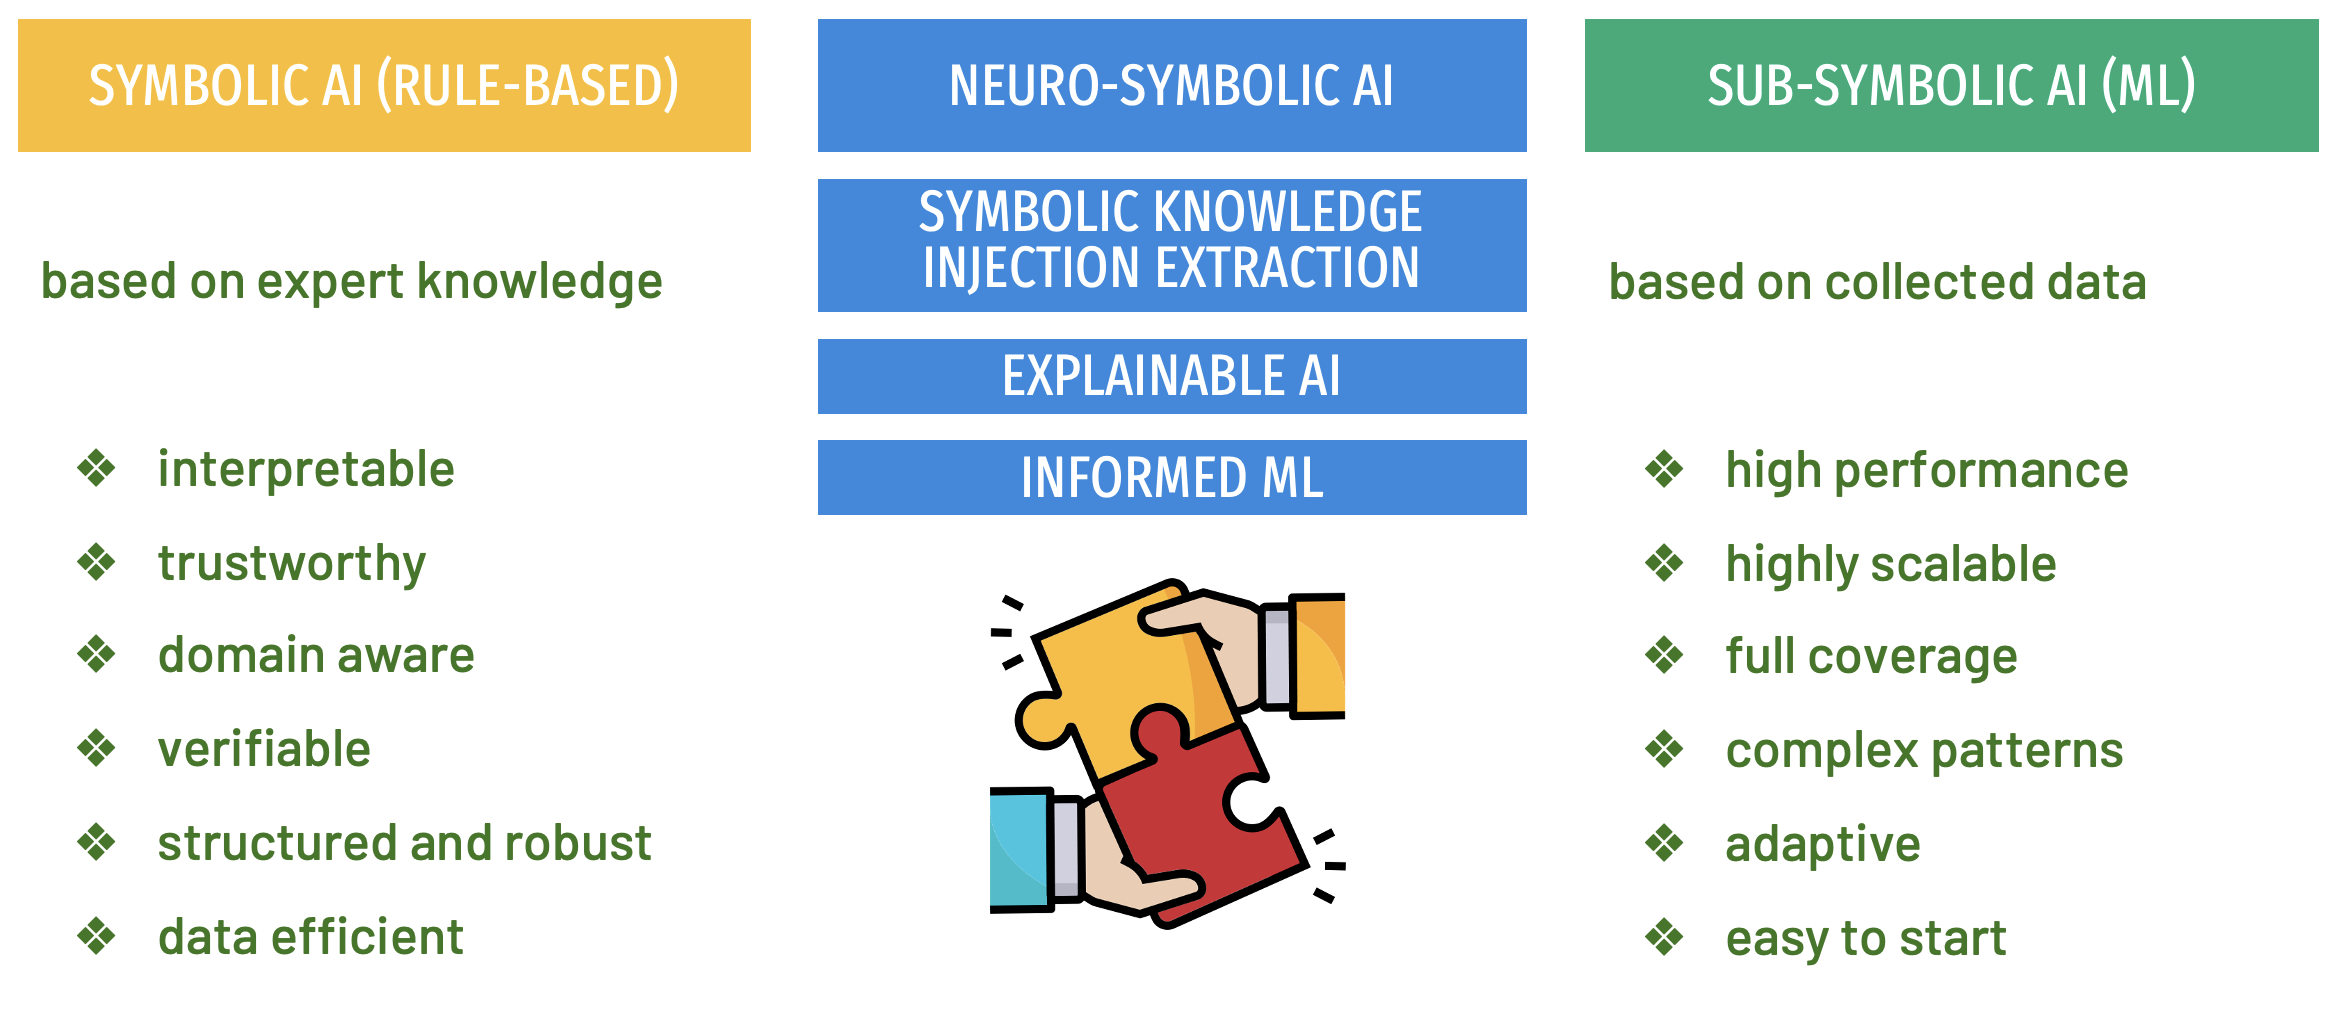
\includegraphics[width=1.0\textwidth]{imgs/conclusion.png} 
 \end{figure} 

\end{frame}
}

%===============================================================================
\section*{}
%===============================================================================
\frame{\titlepage}
{
 \usebackgroundtemplate{}

\setbeamertemplate{page number in head/foot}{}
%\\\\\\\\\\\\\\\\\\\\\
\begin{frame}[t,allowframebreaks,noframenumbering]\frametitle{\refname}
% \begin{frame}[c]\frametitle{\refname}
	\AtNextBibliography{\scriptsize}
	\setlength{\bibitemsep}{.5\baselineskip}
	\printbibliography
\end{frame}}

\end{document}
